\section{Theoretische Vorbereitung}
    \begin{itemize}
        \item für die Sekundärspule ist keine homogene Bewickelung notwendig, warum?
        \item 
    \end{itemize}
    \subsection{Grundlegende Beziehungen}
        \subsubsection{Magnetfelder}
            In der Physik wird das Vektorielle Magnetfeld meist als B-Feld bezeichnet. Es besitzt den Formelbuchstaben
            $\vec{B}$ und wird genauer auch als Magnetische Flussdichte bezeichnet und es wird in der Regel in Tesla angegeben.
            Das B-Feld ist jedoch keine Messbare größe, die zugehörige Messgröße zum B-Feld ist die Magnetische Feldstärke $\vec{H}$.
            Die Magnetische Feldstärke $H$ wird in Ampere pro Meter angegeben ($\frac{A}{m}$) und ist im Vaccum auch Direkt proportional
            zum B-Feld. Dort gilt
            \begin{equation}
                \vec{B} = \mu_0 \vec{H}
            \end{equation}
            $\mu_0$($\eqsim 4\pi ×10^{-7 }\frac{N}{A^2}$) bezeichnet dabei die Magnetische permeabilität von Vaccum.
            In Anwesenheit eines Material mit Magnetisierungs Vektor $M [\frac{A}{m}]$, welcher die dichte der im Material induzierten oder permanenten magnetischen Dipolmomente angibt, ändert sich der Zusammenhand zu
            \begin{equation}
                \vec{B} = \mu_0 (\vec{H} + \vec{M})
            \end{equation}
            Zusätzlich lässt sich nun die magnetische Suszeptibilität $\chi$ nutzen um beispielsweise die Relation zwischen $\vec{H}$ und $\vec{M}$ zu beschreiben
            \begin{equation}
                \vec{M} = \chi \vec{H}
            \end{equation}
            Die magnetische Suszeptibilität beschreibt dabei wie stark dich die Magnetisierung in einem
            Material bei angelegetem Magnetfeld ändert, bzw wie viele der Magnetischen momente sich ausrichten.
            Dabei Unterscheidet man im Allgemeinen zwischen
            \begin{itemize}
                \item $\chi > 0$ Paramagneten
                \item $\chi < 0$ Diamagneten
            \end{itemize}
            Daraus folgt über
            \begin{equation}
                \mu = \mu_0 (1 + \chi)
            \end{equation}
            die Magnetsiche permeabilität $\mu [\frac{N}{A^2}]$, die das Verhältniss zwischen Magnetischer Flussdichte $B$ und magnetischer Feldstärke $H$ beschreibt
            $$ \mu = \frac{B}{H}$$
            Zuletzt gilt es noch das magnetische (Dipol-)Moment $\vec{\mu}$ [$\frac{A}{m^2}$] zu beschreiben, dieses ist ein Maß für die Stärke
            und Richtung eines Magnetischen Dipols. Es lässt sich jedoch auch für Ströme definieren, beispielsweise gilt für eine
            Leiterschleife
            \begin{equation}
                \vec{\mu} = n I \vec{A}
            \end{equation}
            oder Allgemeiner 
            \begin{equation}
                \vec{D} = \vec{\mu} \times \vec{B}
            \end{equation}.
            Erweitert man das Konzept einer Leiterschleife zu einer Reihe derselbigen, erhält das Magnetfeld einer Spule mit Windungen N
            \begin{equation}
                B = N \frac{\mu_0 I}{l}
            \end{equation}
    \subsection{Magnetismus ohne Ordnungsphänomene}
        \subsubsection*{gyromagnetisches Verhältniss}
            das gyromagnetische Verhältnis eines magnetischen Moments wird beschrieben über das Verhältnis
            des magn. Moments und dessen Drehimpuls
            \begin{equation}
                \gamma = \frac{\mu}{L}
            \end{equation}
        \subsubsection*{Spin-,Bahnmagnetismus und Landé-Faktor}
            Alle Teilchen die sowohl einen Drehmoment als auch eine el. Ladung besitzten, haben ein magn. Dipolmoment.
            \begin{equation}
                \vec{\mu_l} = \frac{q}{2m} \vec{l}
            \end{equation}
            dies wird allg. als Bahnmagnetismus beschrieben. Analog dazu gilt eine ähnliche formel für den Spin
            \begin{equation}
                \vec{\mu_s} = \frac{q\cdot g_s}{2m} \vec{s}
            \end{equation}
            bei dem der anomale Spin-g-Faktor berücksichtigt wird.
            Das Bohr'sche Magneton ist der Betrag des magnetischen Moments, welches ein Elektron
            mit $l=1$ erzeugt, also der Grundzustand.
            \begin{equation}
                \mu_B = \frac{e \hbar}{2 m_e} = 5,7883818060(17)\cdot 10^{-5} \frac{eV}{T}
            \end{equation}
            Das magnetische Moment eines Elektrons wird meist durch ein vielfaches des Bohr'schen
            Magneton beschrieben.
            Der Landé-Faktor ist das Verhältnis der Diskrepanz, zwischen dem gemessenen magnetischen Moments
            und dem errechneten (kl. Physik), eines Elektrons. $g_s \approx 2$ für ein Elektron.
        \subsubsection*{Diamagnetismus}
            Bei einem Diamagneten richten sich die inneren magnetischen Momente entgegengesetzt
            zu einem äußeren Magnetfeld aus. Dies passiert auf Grund der unten erklärten Lenz'schen Regel.
            Außerhalb eines magnetischen Feldes sind Diamagneten
            nicht magnetisch. Der einzige ideale Diamagnet ist ein Supraleiter, bei denen gilt $\chi = -1$           
        \subsubsection*{Lenz'sche Regel}    
            Die Lenz'sche Regel besagt, dass eine Änderung eines Magnetfeldes $\vec{B}$ einem der Änderung
            entgegenwirkenden Strom induziert
        \subsubsection*{Langevin-Gleichung}
            \hl{fehlt alles}
            Stochaistische Differentialgleichung oder so 
        \subsubsection*{Paramagnetismus}
            Ein Paramagnet besitzt eine positive Suszeptibilität, ist jedoch ohne äußeres 
            Magnetfeld nicht magnetisch. In einem Paramagneten richten sich die inneren magnetischen 
            in Richtung des Feldes aus.
            \hl{Beitraege}
            Der Pauli-Paramagnetismus entsteht durch freie Elektronen in Metallen, die über ihren Spin 
            in magnetisches Moment besitzen. Da jedoch, aufgrund des Pauli-Prinzips, nur angeregte
            Leitungselektronen über der Fermi Energie sich nach dem Magnetfeld ausrichten können, 
            ist die Anzahl der beitragenden Elektronen proportional zur Materialabhängigen Fermi-Temperatur.
            \begin{equation}
                \chi_{Pauli} \thicksim \frac{C}{T} \cdot \frac{T}{T_{F}} = \frac{C}{T_F}\thicksim 10^{-6 ... -5}
            \end{equation}
            mit C der Curie-Konstante, T der Temperatur und $T_F$ der Fermi-Temperatur.
    

    \subsection{Magnetismus mit Ordnung}
        \subsubsection*{Wechselwirkung}
            Die Magnetische Ordnung kommt zustande über die sogennante Austauschwechselwirkung, bei welcher sich
            die atomaren Gesamtdrehmomente einem Energietischen minimum erstrebend zueinander Ausrichten. Dabei ist 
            das Pauli-Prinzip ein entscheidener Faktor, da durch dieses bei Fermionen viele der Übergänge verboten sind.
            Ein häufig verwendetes modell um diese Austauschwechselwirkung zu beschreiben ist das s.g. Ising-Modell.
        \subsubsection*{Anisotropie}
            Magnetisch leichte Achsen bzw Schwere Achsen beschreiben Achsen entlang denen die Magnetisierung bevorzugt
            bzw. nur unter großem Aufwand stattfindet. Die Anisotropieenergie bezeichnet dabei die notwendige Energie
            um eine Magnetisierung von einer Leichten in eine schwere Achse zu drehen.\\
            Anisotropieenergie spaltet sich dabei grob in 3 Terme auf
            \begin{itemize}
                \item \textbf{Magnetokristalline Anisotropie}, hervorgerufen durch die Anisotropie einer Kristallstruktur
                \item \textbf{Formanisotropie}, resultierend aus der Probengeometrie
                \item \textbf{induzierte Anisotropie}, durch spannungen aufgrund von unregelmässigkeiten. 
            \end{itemize}
        \subsubsection*{Ferro-, Ferri-, Antiferromagnetismus}
            Ferromagneten Zeichnen sich darüber aus, dass sich sog. Weissersche Bezirke bilden, in diesen Bezirken
            kommt es zu einer Spontanten Magnetisierung der magn. Dipole. Das bedeutet, dass sich die Dipole entlang einer
            gemeinsamen Vorzugsrichtung ausrichten. Dieses Verhalten kann spontan und unabhängig von einem äusseren Magnetfeld
            auftreten, wird es jedoch durch ein solches induziert bleibt es auch in abwesehnheit eines solchen bestehen.
            Beim Ferrimagnetismuss verhält es sich recht Analog, jedoch sind einige Dipole entgegengesetzt ausgerichtet.
            Dabei kommt es jedoch nicht zu einer aufhebung der Magnetisierung, da in Ferrimagnetischen Materialen
            eine Ausrichtung bevorzugt d.h. Stärker ist, wodurch eine Gesamtmagnetisierung entsteht. 
            Bei Antiferromagnetischen Materialen vergält es sich wie bei Ferrimagnetischen Materialen ohne Vorzugsrichtung,
            wodurch sich keine Magnetisierung durchsetzt, es bleibt unmagnetisch.
            \begin{figure}[H]
                \centering
                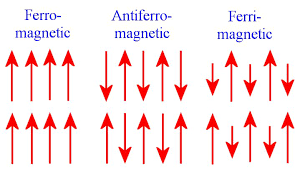
\includegraphics{Images/ferroferrianti.png}
            \end{figure}
        \subsubsection*{Ferromagnetismus}
            Wie bereits angesprochen kommt es in Ferromagnetischen Materialien zu sog. Weiss'sche Bezirke,
            oder auch Domänen, bilden sich aufgrund der Kristallstruktur und dessen inhomogenitäten, dabei 
            hängt die Vorzugsrichtung des jeweiligen Bezirks von dem Kristallgitter der Probe ab. Solche 
            Bezirke erstrecken sich von etwa 10 bis 1000$\mu m$ in linearer Ausdehnung.\\
            An den Übergängen von zwei Weiss'schen Bezirken kommt es zu sog. 
            \hl{todo: Energie, Wandversch., Drehung, Barkhausenspruengen, Reversibilitaet}
        \subsubsection*{Hysteresekurve}
            Hysteresenkurven treten in vielen Bereichen der Physik auf, in diesem Fall wird jedoch die Magnetisierung
            der Probe in abhängigkeit eines äusseren Feldes aufgetragen.\\
            Führt man eine Solche Messung durch beginnt der Graph mit der sogennanten Neukurve, dabei richten sich
            die Weiss'schen Bezirke das erste mal aus bis zum Punkt der Sättigung. Misst man dann die Magnetisierung bei einem Abnehmenden Magnetfeld
            kommt man zunächst zum Remanenzfeld, welches bestehenbleibt obwohl kein äusseres Feld mehr angelegt ist, bis 
            das Koerzitivfeld erreicht ist, und es erneut zur spontanen Magnetisierung kommt und der Vorgang von neuem Beginnt.
            \begin{figure}[H]
                \centering
                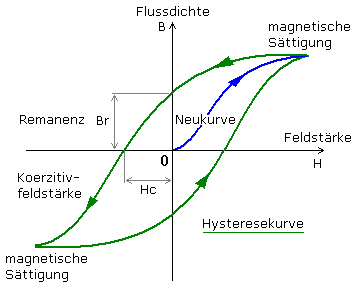
\includegraphics[width=0.9\textwidth]{Images/hyster.png}
                %https://www.google.com/url?sa=i&url=https%3A%2F%2Fwww.elektroniktutor.de%2Felektrophysik%2Fmagkurve.html&psig=AOvVaw202TVqiaXyCzzC35HNuQiG&ust=1622981447740000&source=images&cd=vfe&ved=0CAMQjB1qFwoTCLi505e7gPECFQAAAAAdAAAAABAD
            \end{figure}

            Zeigen Sie, dass der Fl ̈acheninhalt der Hysteresekurve ein Maß f ̈ur die Energie ist, diebeim einmaligen Umfahren der Kurve als W ̈arme auftritt (Verlust).Je h ̈oher die Energie, die aufgebracht werden muss um die Weißschen Bezirke auszu-richten, desto gr ̈oßer ist die Remanenz und Koerzitivfeldst ̈arke. Und je gr ̈oßer Remanenzund Koerzitivfeldst ̈arke, desto gr ̈oßer die Fl ̈ache unter der Hysteresekurve. Daraus folgt,Der Fl ̈acheninhalt ist proportional zur ben ̈otigten Energie, die beim einmaligen Umfah-ren der Kurve ben ̈otigt wird
        \subsubsection*{magn. Hart und Weich}
            Magnetisch weiche Stoffe zeichen sich durch eine besonders leichte Magnetisierbarkeit aus, das bedeutet,
            dass sie eine kleineres Koerzitivfeld benötigen um ihre Magnetisierung zu ändern. Anders ist es bei Harten
            magnetischen Stoffen bei denen die Magnetisierung besonders Schwer ist.
            \begin{figure}[H]
                \centering
                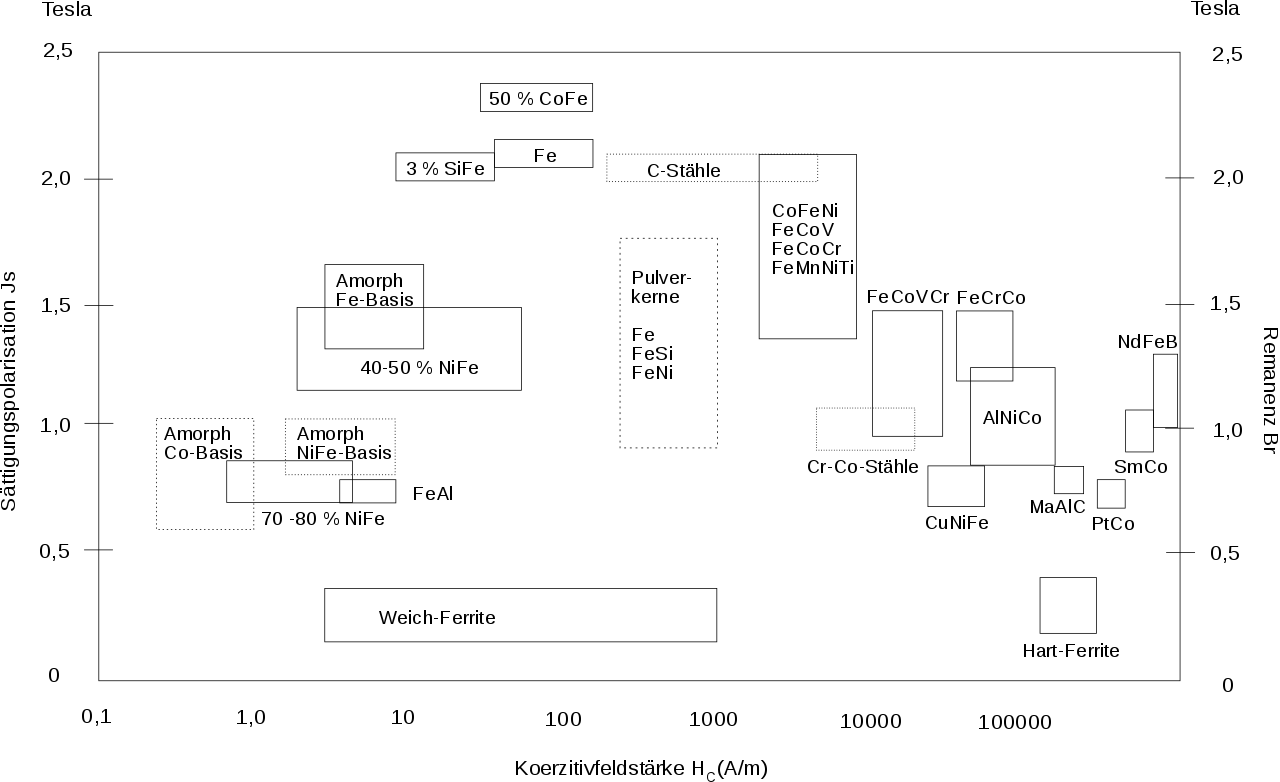
\includegraphics[width=0.9\textwidth]{Images/Übersicht_Koerzitivfeldstärke.png}
                %https://de.wikipedia.org/wiki/Magnetwerkstoffe#/media/Datei:%C3%9Cbersicht_Koerzitivfeldst%C3%A4rke.svg
            \end{figure}
        \subsubsection*{Ferrite}
            
        \subsubsection*{Temperatureinfluss}
            Bei steigenden Temperaturen führt die thermische Energie zu bewegung im Material, wodurch die Ordnung der
            Dipole gestört wird. Je höher die Temperatur desto schwerer wird es für die Dipole ihre Ausrichtung entlang 
            der Feldlinien bei zubehalten. Steigt die Temperatur über die sog. Curie Temperatur verliert das Material
            die Eigenschaft der Magn. Ausrichtung und wird nichtmagnetisch 
        \subsubsection*{Phasenübergang}
            %https://sci-hub.se/https://link.springer.com/chapter/10.1007/978-3-642-82138-7_1
            Bei Thermondynamischen Phasenübergänge spricht man häufig über eine Spontane Änderung der Freien Energie F.
            Bei ihnen wird zwischen Übergängen erster und zweiter Ordnung Unterschieden. Übergänge erster Ordnung
            arbeiten mit latenter Wärme, also ohne Temperaturänderung. Dabei tauscht das System eine Feste menge an energy
            mit der Umgebung aus.\\
            Bei übergängen 2ter ordnung ist keine solche spontanität zu erkennen, sie sind auch sog. Kontinuierliche Phasenübergang
            \begin{figure}[H]
                %https://en.wikipedia.org/wiki/Phase_transition
                \centering
                \includegraphics[width=0.9\textwidth]{Images/waterphase.png}
            \end{figure}
    \subsection{Entmagnetisierungsfaktor}

        \subsubsection*{Entmagnetisierung}
            Eine Entmagnetisierung ist ein Vorgang, indem das Magnetfeld eines Magneten verschwindet.
            Die Ursache hierfür können: Erschütterung, Hitze sein. Aber meist wird ein Material
            durch ein zuerst starkes Wechsel-Magnetfeld, welches aber mit der Zeit abklingt, verwendet.
            \hl{Bild}
            \begin{figure}[H]
                \centering
                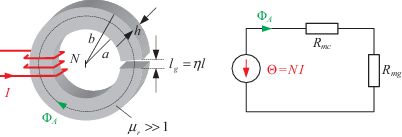
\includegraphics{images/Ringkern}
            \end{figure}
        \subsubsection*{Herleitung Entmagnetisierungsfaktor}
            Man nimmt an, dass die Lücke des Rings sehr klein ist und die Feldlinien sich homogen
            fortsetzen. Dann vergleicht man die Erregerfelder mit und ohne Luftspalt. Dies geht, da 
            bei beiden die gleiche Stromstärke verwendet wird.
            \begin{equation}
                H \cdot L = H_R \cdot L_R + H_L \cdot L_L
            \end{equation}
            mit $L = 2 \pi r$ der Umfang des Kerns. $L_L, L_R$ sind die Länge der Lücke bzw. des restlichen Kerns.
            $H_R, H_L$ sind die Erregerfelder im Ring und in der Lücke.
            Mit den Maxwellgleichungen und dem Stoke'schen Satz folgt:
            \begin{equation}
                B_R \cdot F = B_L \cdot F
            \end{equation}
            mit F ist die Querschnittsfläche des Rings. Es gilt allg.
            \begin{equation}
                B = \mu_0 (H + M)
            \end{equation}
            da Luft als Vakuum genähert werden kann, ist $M=0$ in der Lücke.
            Durch diese Gleichungen ergeben sich für $H_R$ bzw. $H_L$:
            \begin{align*}
                H_R = H - \frac{L_L}{L} M\\
                H_L = H + \frac{L_L}{L} M
            \end{align*}
            das entmagnetisierende Feld ist damit:
            \begin{equation}
                H_e = \frac{L_L}{L} M 
            \end{equation}
            mit dem Entmagnetisierungsfaktor $N = \frac{L_L}{L}$
        \subsubsection*{gescherte Hysteresenkurven}
            %https://www.google.com/url?sa=i&url=https%3A%2F%2Fsilo.tips%2Fdownload%2Fmagnetisierungskurven-eines-ferrits-1&psig=AOvVaw1-iHGdJClryjKD8ByJthm3&ust=1623062593991000&source=images&cd=vfe&ved=0CAIQjRxqFwoTCMjA4MHpgvECFQAAAAAdAAAAABAO
            das entmagnetisierende Feld $H_{ent}$ immer großer wird, werden wir das erzeugende Feld $H_{ohne}$ 
            auchsteigern müssen. Wenn man in einem M-H-Diagramm eine Hysterese für einen Ringkern
            ohne Luftspalt aufnimmt, so ist $H_{ent}=H_{ohne}$. Für Hyteresen mit Ringkernen,
            die einen Luftspalt besitzen, steigen die $H_{ohne}$-Werte, die die gleiche Magnetisierung
            bzw. das gleiche $_{ent}$ erzeugen, immer weiter an, sodass die Hysterese nach rechts
            geschert wird. Man nennt diese Hysteresen daher auch gescherte Hysteresen.
            \begin{figure}
                \centering
                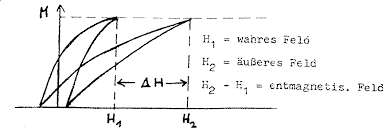
\includegraphics[width=0.9\textwidth]{Images/geschert.png}
            \end{figure}
            
        \subsubsection*{Einfluss der Entmagnetisierung auf $\chi$}

            
